\documentclass[11pt, oneside]{article} 
\usepackage{geometry}
\geometry{letterpaper} 
\usepackage{graphicx}
	
\usepackage{amssymb}
\usepackage{amsmath}
\usepackage{parskip}
\usepackage{color}
\usepackage{hyperref}

\graphicspath{{figures/}}
% \begin{center} \includegraphics [scale=0.4] {gauss3.png} \end{center}

\title{Ptolemy's theorem}
\date{}

\begin{document}
\maketitle
\Large

%[my-super-duper-separator]

Ptolemy was a Greek astronomer and geographer who probably lived at Alexandria in the 2nd century AD (died c.168 AD).  That is nearly 500 years after Euclid.  (Ptolemy was a popular name for Egyptian pharaohs in earlier centuries).

Our Ptolemy is known for many works including his book the \emph{Almagest}, and important to us here, for a theorem in plane geometry concerning cyclic quadrilaterals.  These are 4-sided polygons with all four vertices on the same circle.  

Recall that any triangle lies on a circle, so this is a restriction on the fourth vertex of the polygon.
\begin{center} 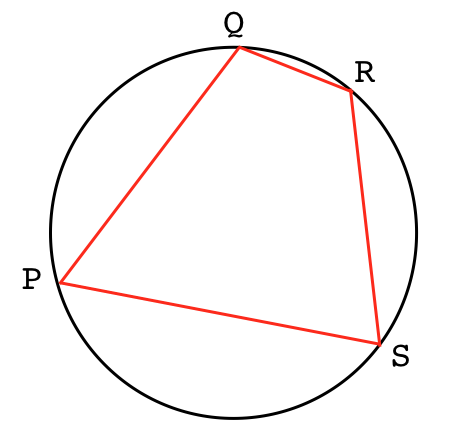
\includegraphics [scale=0.35] {circles_4.png} \end{center}

Also recall the \hyperref[sec:quadrilateral_supplementary]{\textbf{quadrilateral supplementary theorem}} (Euclid III.22):

$\bullet$ \ For \emph{any} quadrilateral whose four vertices lie on a circle, the opposing angles are supplementary (they sum to $180^\circ$).

Now, draw the diagonals $AC$ and $BD$.  Ptolemy's theorem says that if we take the products of the two pairs of opposing sides and add them, the result is equal to the product of the diagonals.
\begin{center} 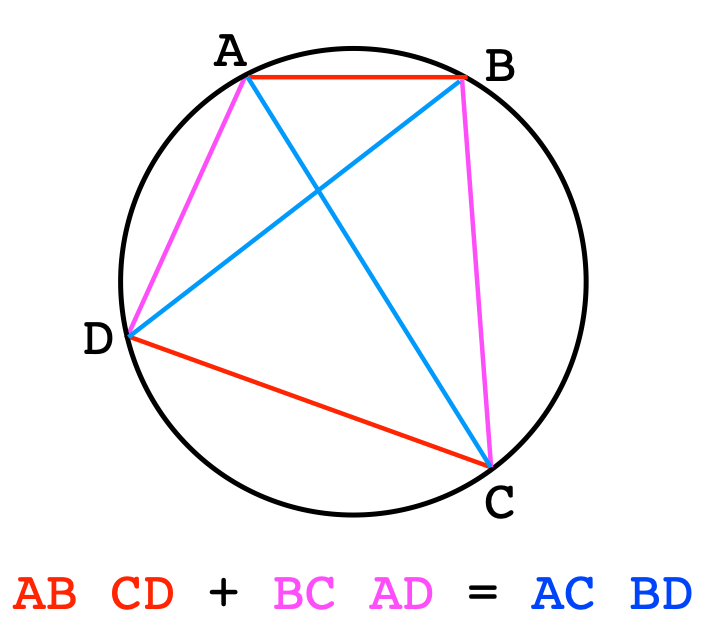
\includegraphics [scale=0.6] {pt1.png} \end{center}
 
\emph{Proof}.

We're going to do a famous dissection of a cyclic quadrilateral as a proof of Ptolemy's theorem, but as a twist on the usual approach we'll do it in reverse, starting with a a parallelogram.  I'm hoping this will make the whole thing clearer.

\begin{center} 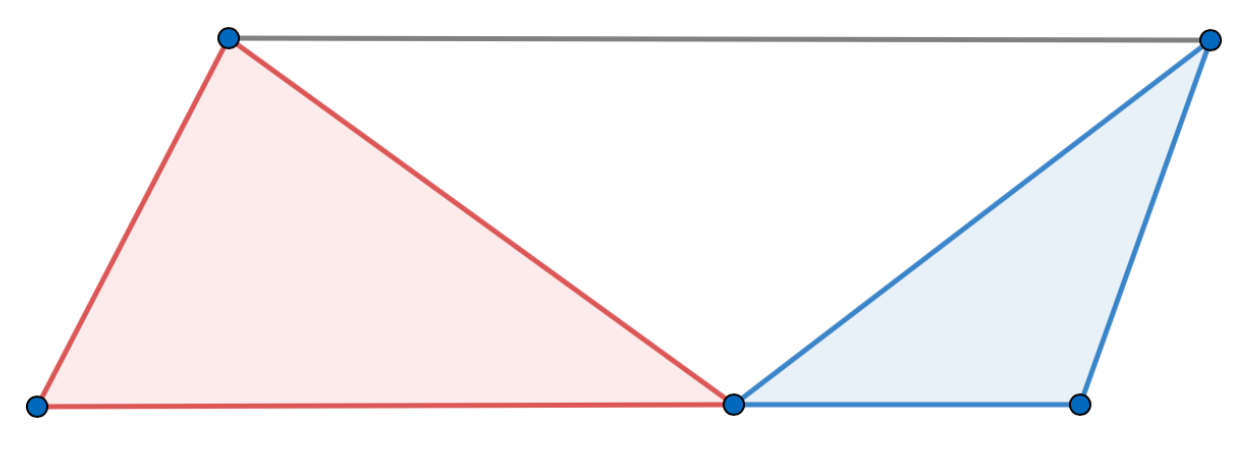
\includegraphics [scale=0.2] {Ptol1.png} \end{center}

We have a parallelogram, and we've picked a point along the bottom edge and drawn lines to the opposing vertices.  Let's label some angles.

\begin{center} 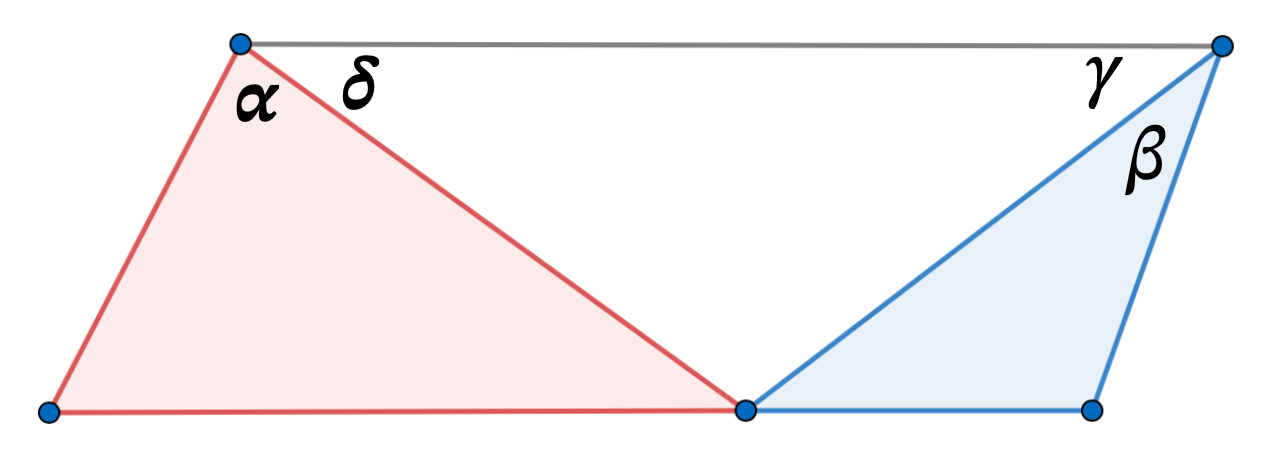
\includegraphics [scale=0.2] {Ptol2.png} \end{center}

And then use the properties of parallels to get the rest of them labeled as well.
\begin{center} 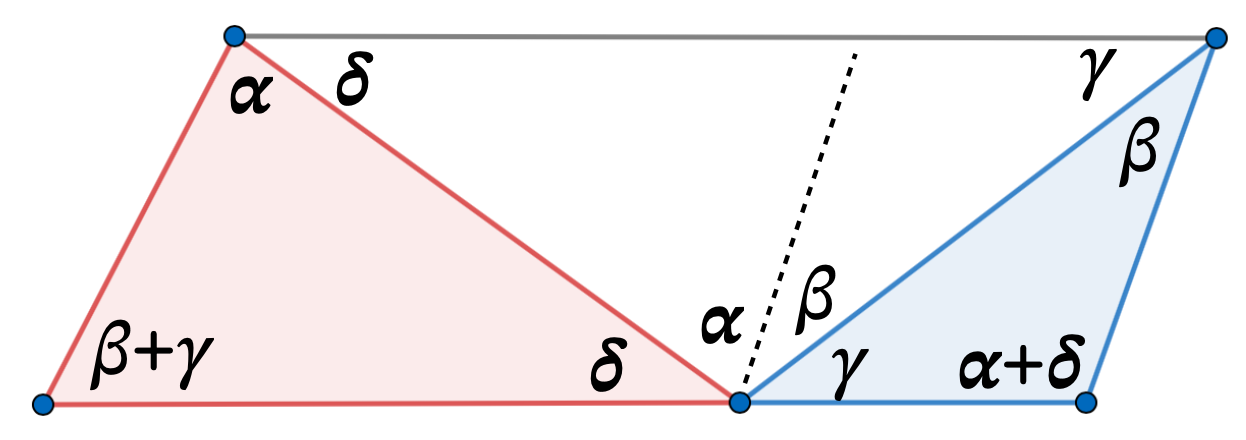
\includegraphics [scale=0.2] {Ptol3.png} \end{center}

As a parallelogram, we have opposing angles equal, and adjacent angles summing to 180 as they must for parallel lines.

Now do the dissection.  Cut out the red triangle and the blue triangle and join them as shown.  In general, the scale will have to be adjusted so that they form a quadrilateral with that edge as the diagonal.  We'll return to this point in a minute.
\begin{center} 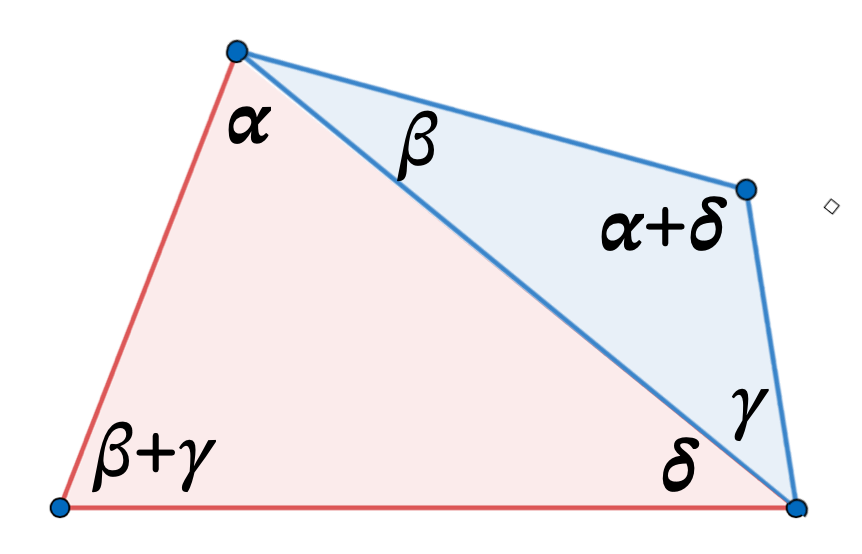
\includegraphics [scale=0.2] {Ptol4.png} \end{center}

This is a cyclic quadrilateral, by the converse of the theorem on cyclic quadrilaterals, since opposing angles are supplementary.
\begin{center} 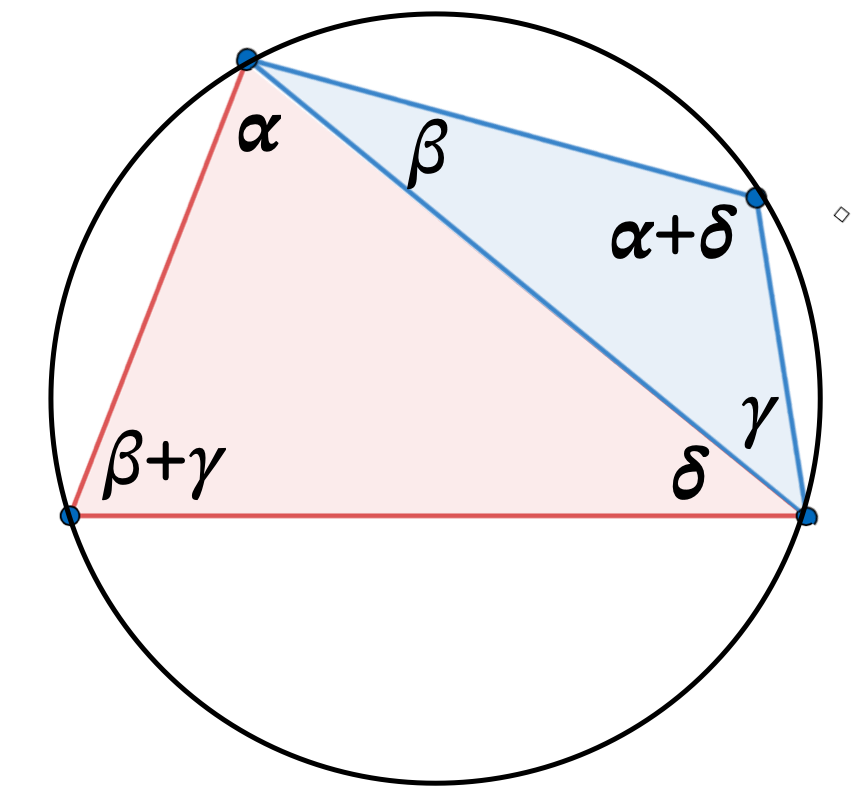
\includegraphics [scale=0.2] {Ptol5.png} \end{center}

We can use the corollary of the inscribed angle theorem to draw the other diagonal and assign angles.
\begin{center} 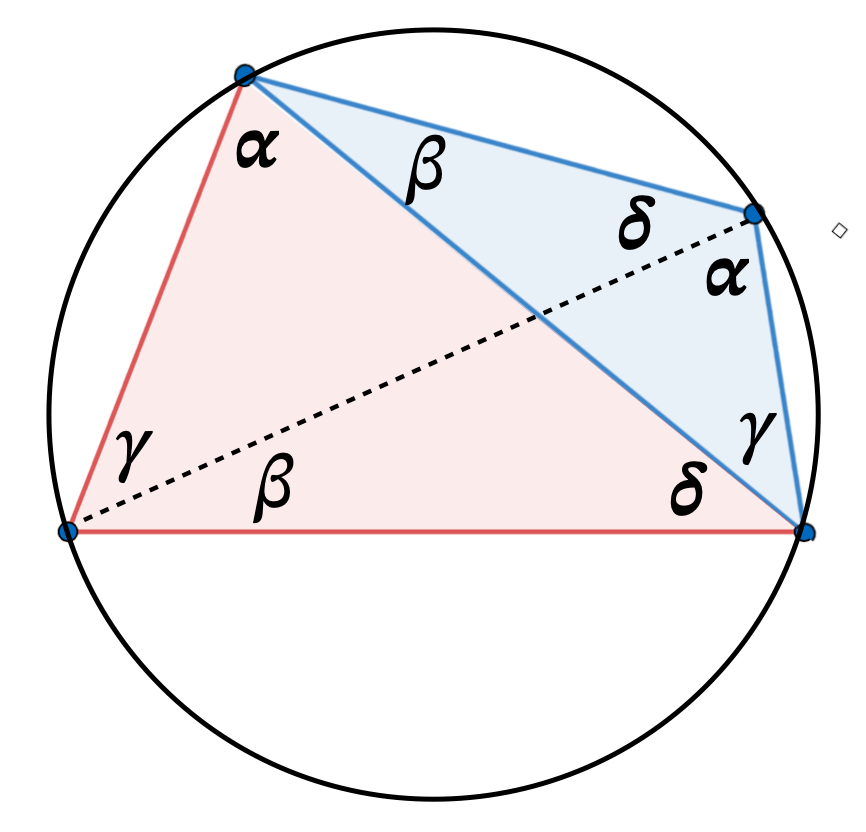
\includegraphics [scale=0.2] {Ptol6.png} \end{center}

We're going switch our attention to the lengths of the sides and diagonals, but before we do, notice a very special triangle (partly red and partly blue) with angles $\gamma, \delta,$ and $\alpha + \beta$.  

That triangle has sides $a, d$ and $y$.
\begin{center} 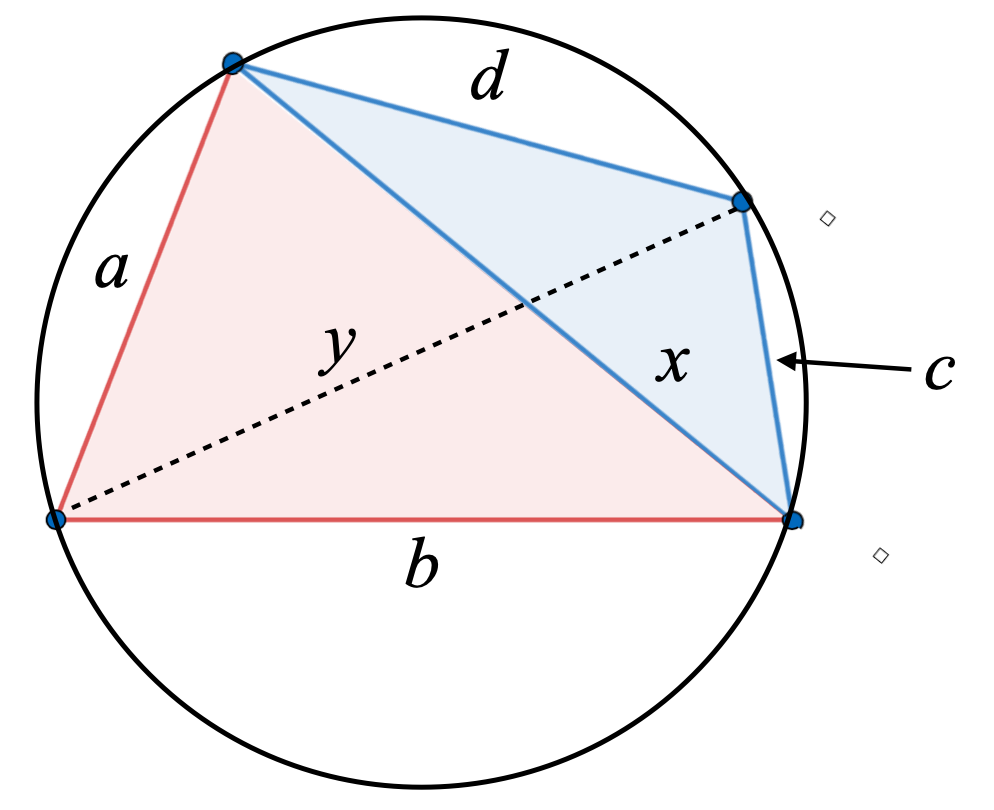
\includegraphics [scale=0.2] {Ptol7.png} \end{center}

Let's reverse the process, dissecting the cyclic quadrilateral by cutting along the $x$ diagonal, and arranging the pieces so that the bases are collinear as in the original parallelogram.

\begin{center} 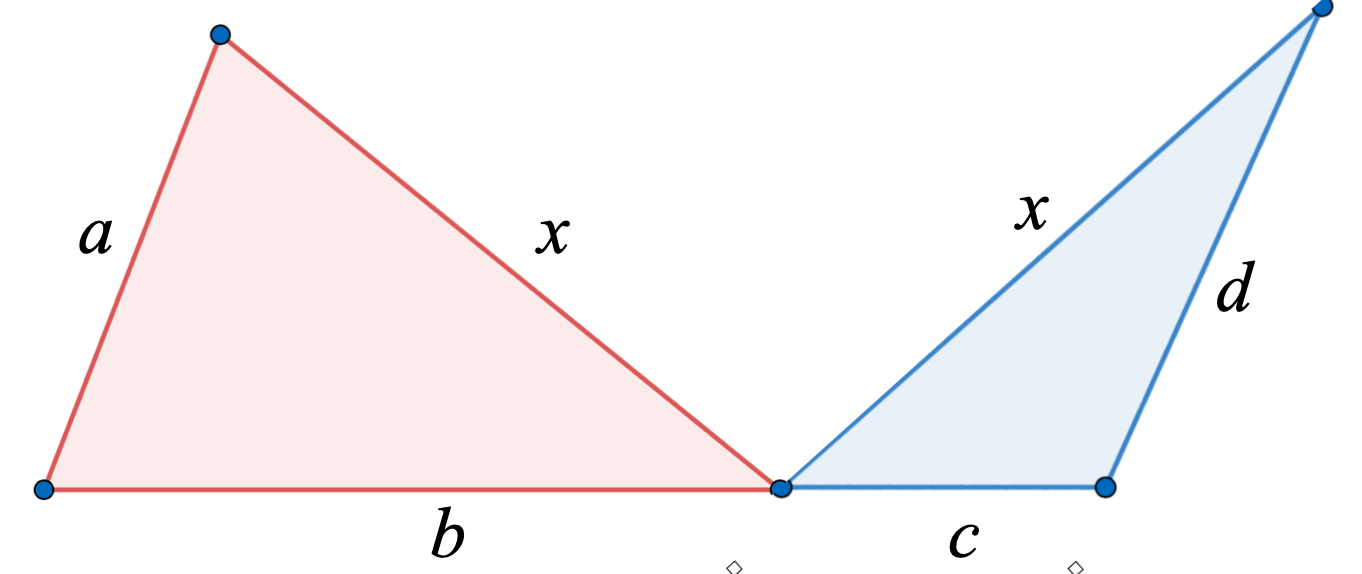
\includegraphics [scale=0.2] {Ptol8.png} \end{center}

In the general case, $a \ne d$.  But we can scale the two sides to be equal.  An easy way to do that is to cross multiply.

\begin{center} 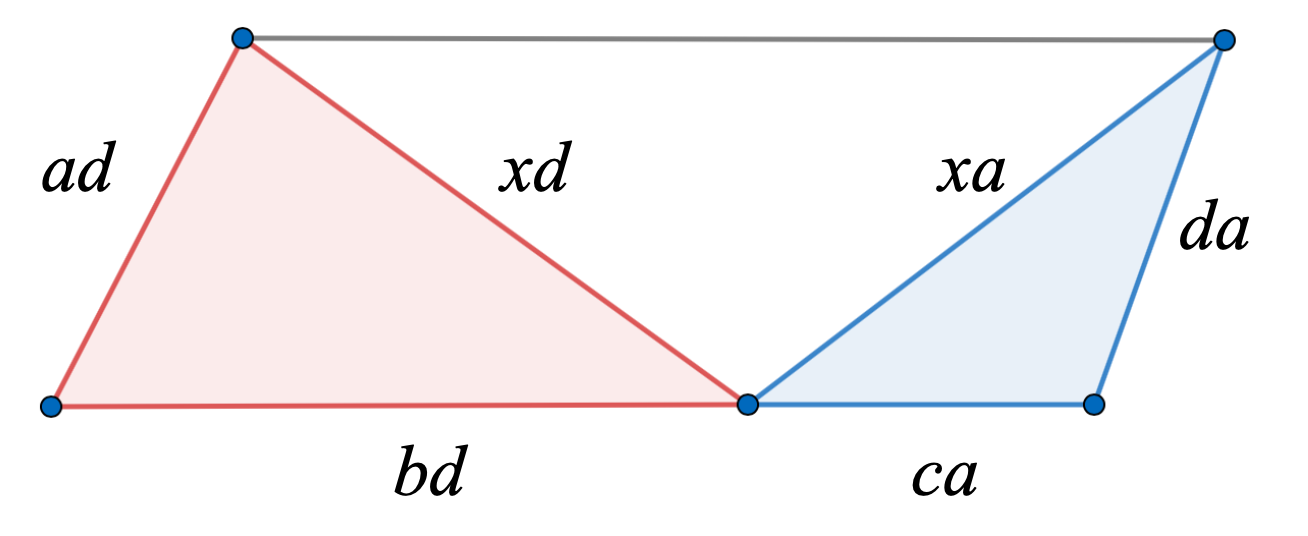
\includegraphics [scale=0.2] {Ptol9.png} \end{center}

We have a parallelogram again.  The angles are correct, and now the sides are equal.  So are the top and bottom equal.  We focus now on the white triangle.

\begin{center} 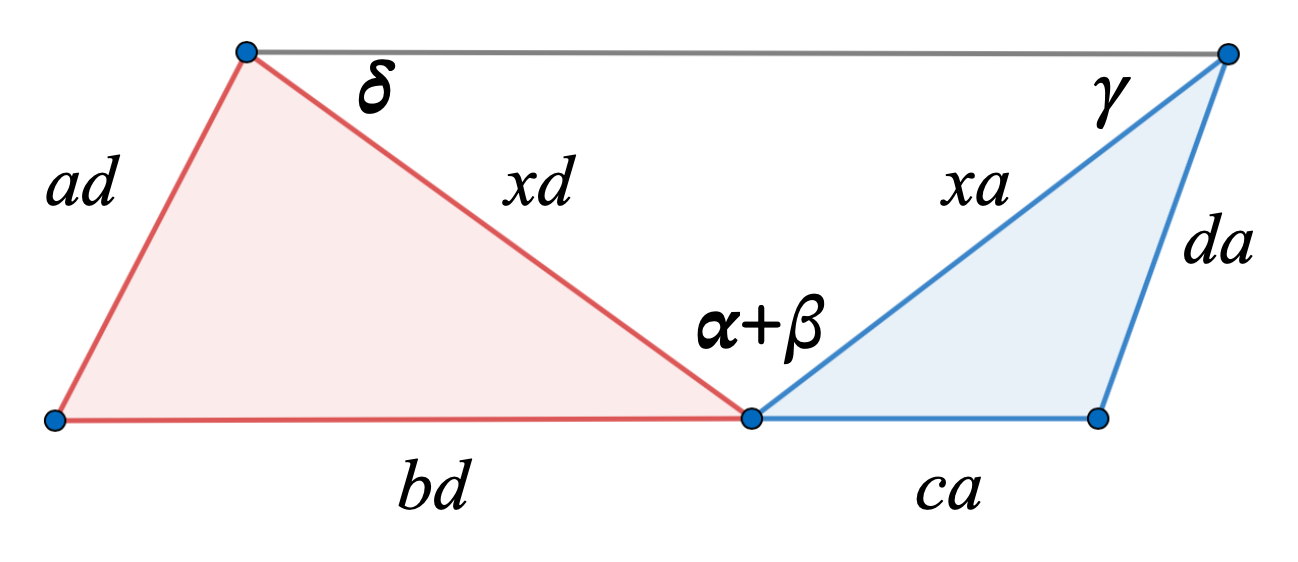
\includegraphics [scale=0.2] {Ptol10.png} \end{center}

It has two sides with lengths $a$ and $d$, each scaled by a factor of $x$, and the two angles opposite those sides are $\delta$ and $\gamma$.

Remember the special triangle?
\begin{center} 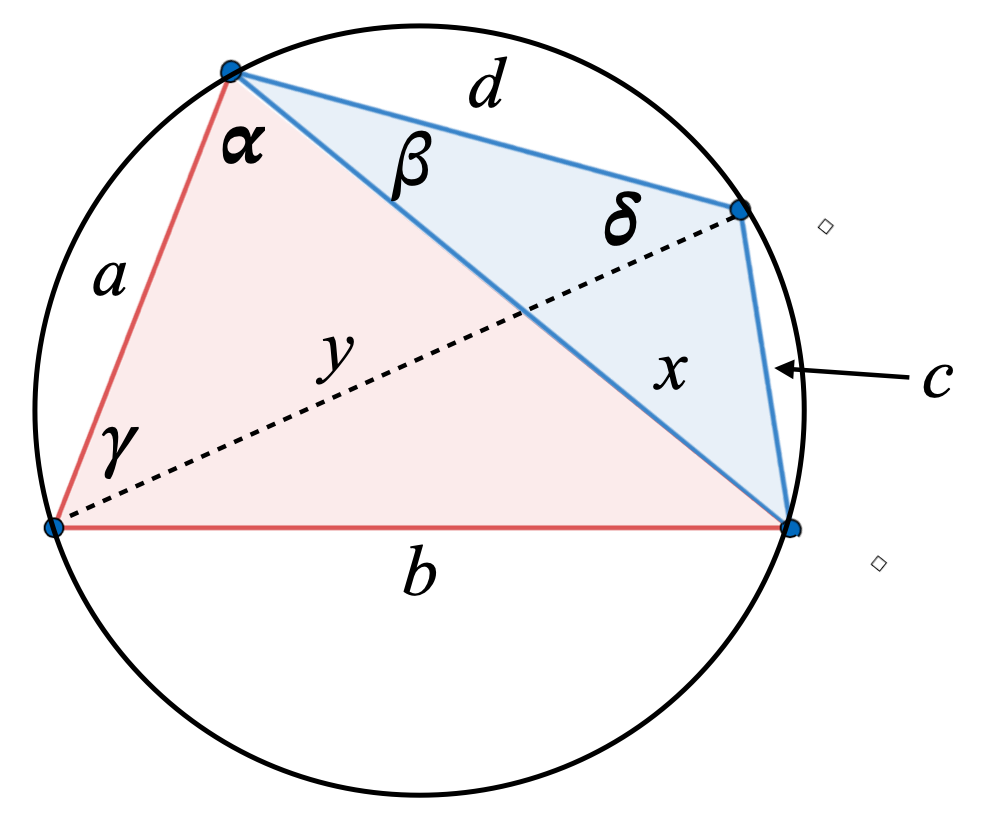
\includegraphics [scale=0.2] {Ptol12.png} \end{center}

We can see it in the cyclic quadrilateral.  The sides are $a,d,y$.  In the parallelogram, that white triangle must be scaled by a factor of $x$, giving sides $xa, xd $ and $xy$.
\begin{center} 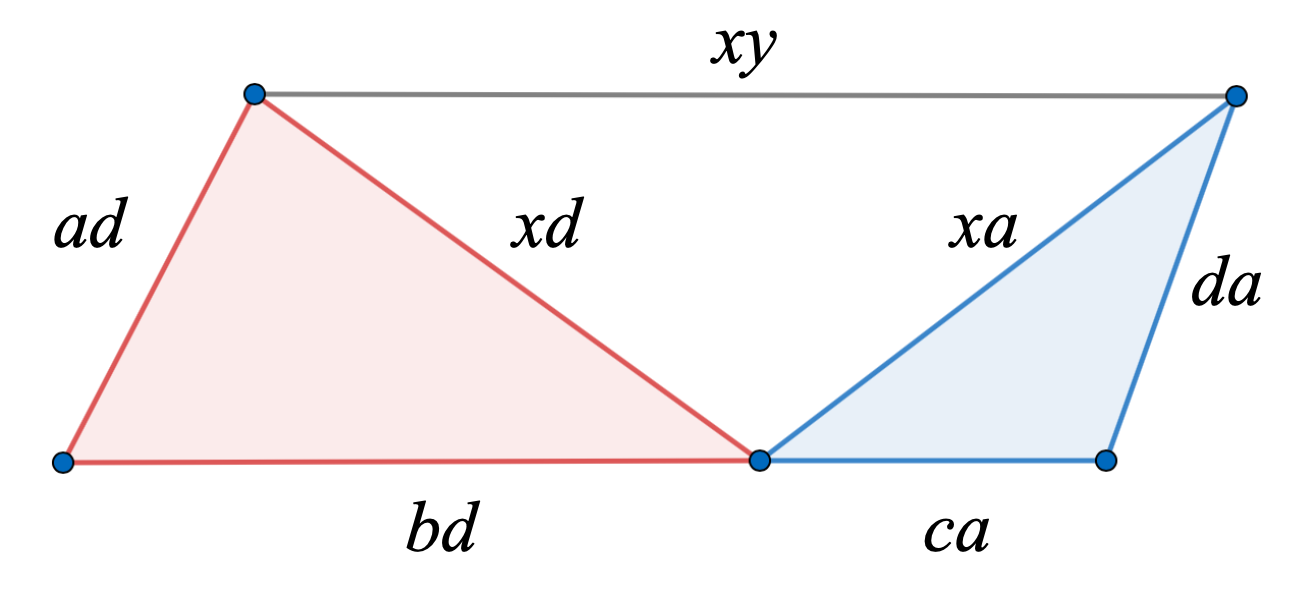
\includegraphics [scale=0.2] {Ptol13.png} \end{center}

Since this is a parallelogram, the top and bottom are equal.  Namely, $ac + bd = xy$.

This is Ptolemy's theorem.

$\square$

I just love that proof.  But admittedly, it is a bit long-winded.  So here is another one.

\subsection*{Ptolemy proof 2}

\begin{center} 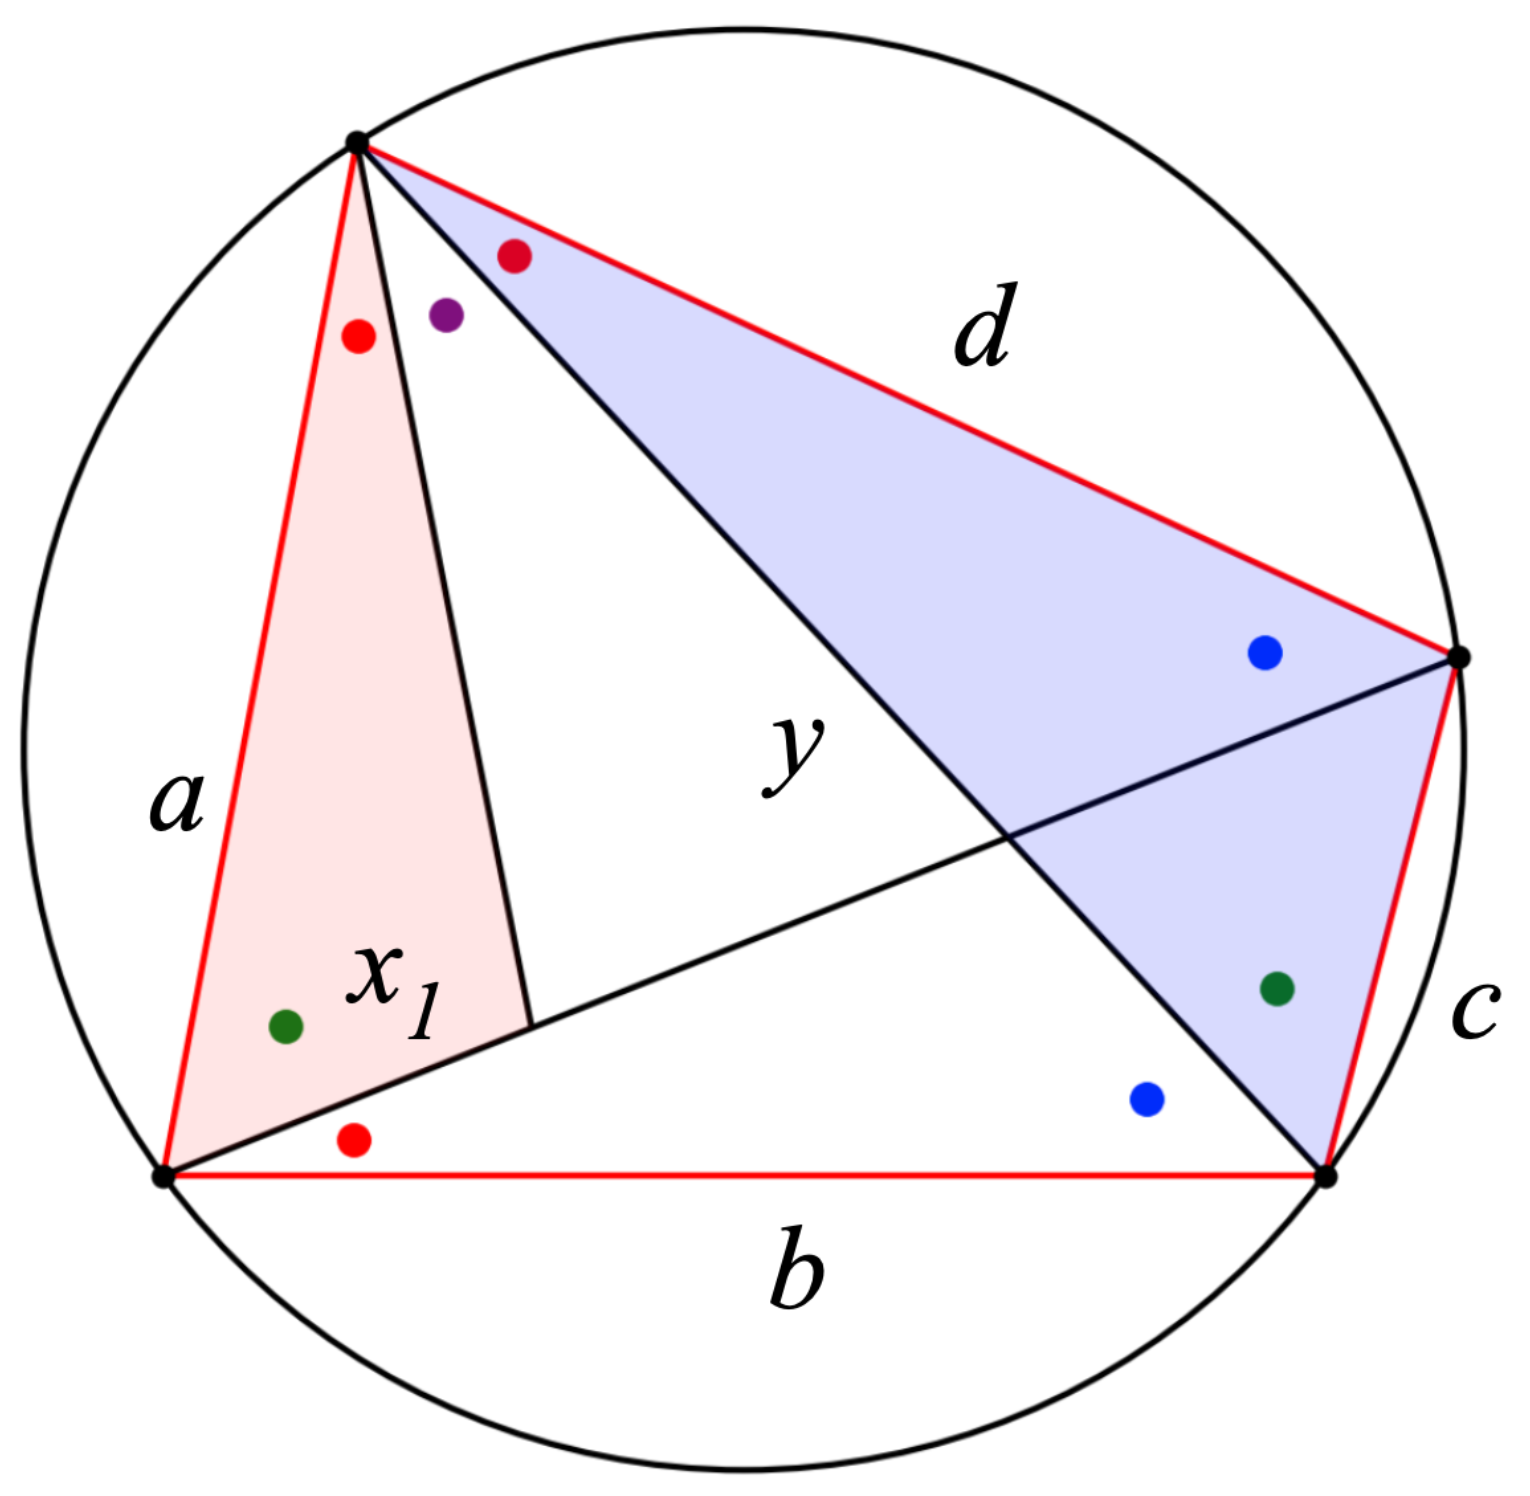
\includegraphics [scale=0.25] {ptolemy_angles1.png} \end{center}

Consider the cyclic quadrilateral in the figure.  Pick one vertex, for example at upper left with diagonal $y$, and subdivide to form the same angle again (red dots), plus the excess (purple dot).

This forms two similar triangles in red and blue, with equal angles marked with red dots, plus another pair of angles marked green, since they both lie on the chord $d$.  We divide the second diagonal into two parts:  $x = x_1 + x_2$.  By similar triangles we have
\[ \frac{x_1}{a} = \frac{c}{y} \]

[If you need to remember this, we are looking to eventually get a term of $xy$.]

\begin{center} 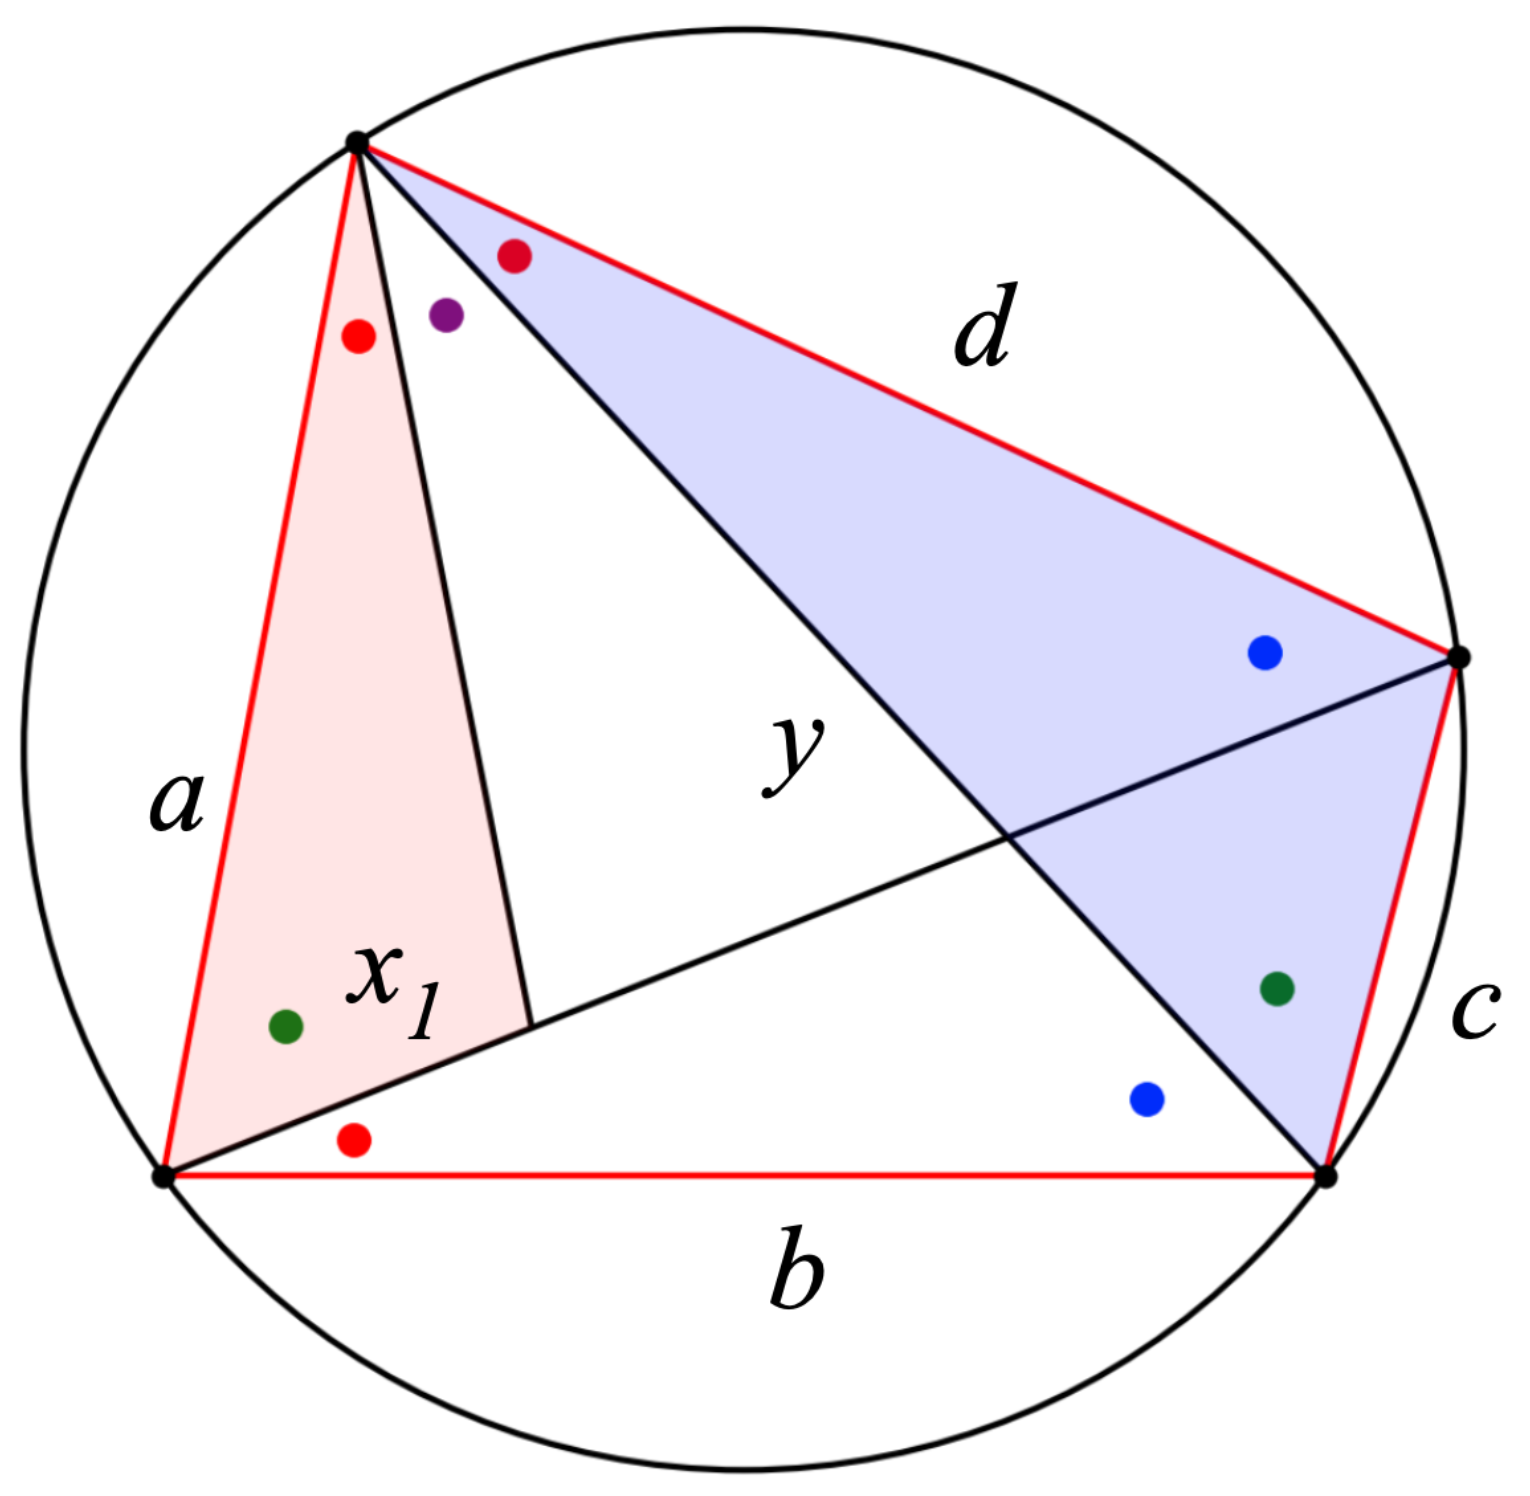
\includegraphics [scale=0.25] {ptolemy_angles1.png} 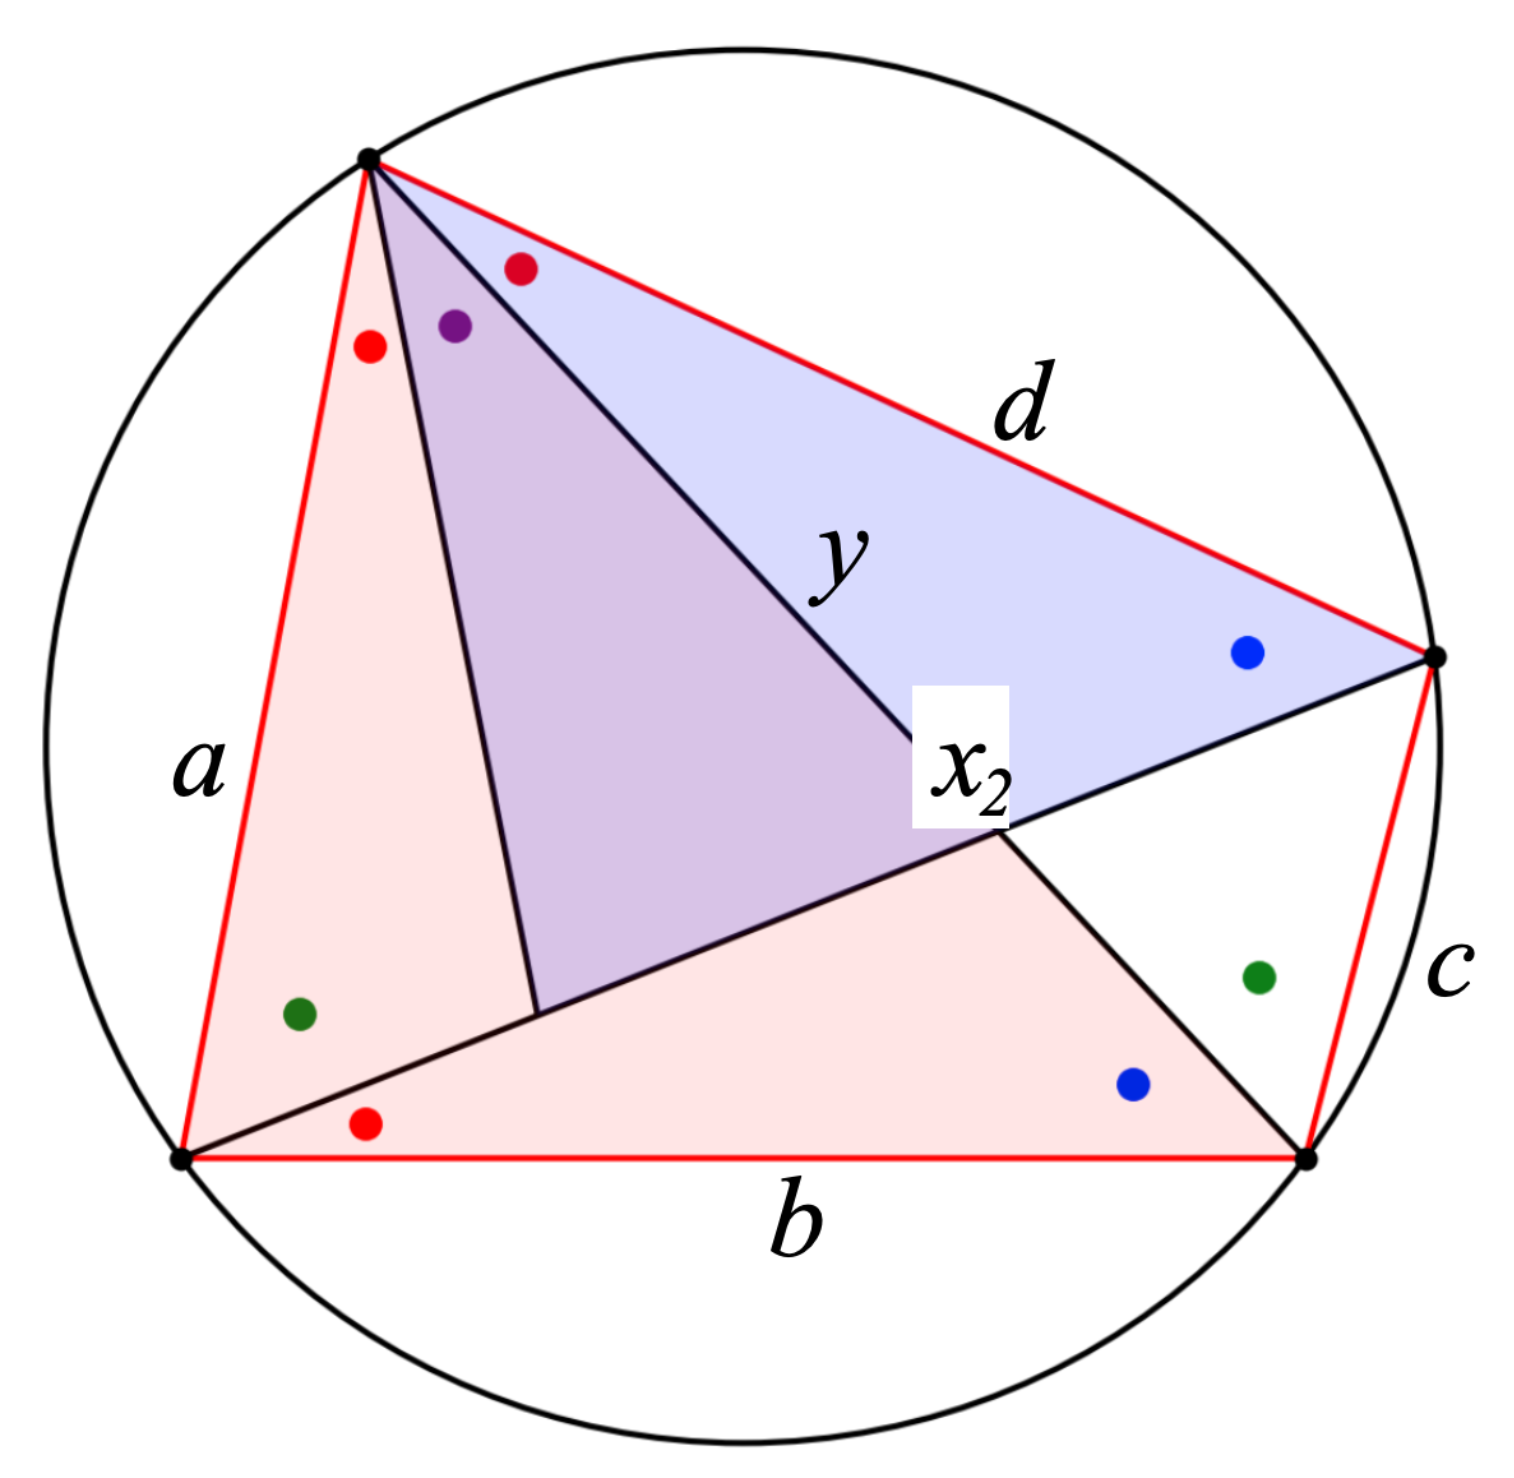
\includegraphics [scale=0.25] {ptolemy_angles2.png} \end{center}

We get another pair of similar triangles with apex angle equal to red \emph{plus} purple.  We need ratios involving $b$ and $d$ as well as $y$ and $x_2$.  I see
\[ \frac{x_2}{d} = \frac{b}{y} \]
which is confirmed by checking the angles opposing the corresponding sides.

We rearrange to obtain
\[ x_1 = \frac{ac}{y} \ \ \ \ \ \ \ \ x_2 = \frac{bd}{y} \]
\[ x_1 + x_2 = x = \frac{ac}{y} + \frac{bd}{y} \]
\[ xy = ac + bd \]

\subsection*{consequences}

Ptolemy's theorem gives a very easy proof of the Pythagorean theorem.

It also provides entertaining proofs of the sum of angles formulas.

\begin{center} 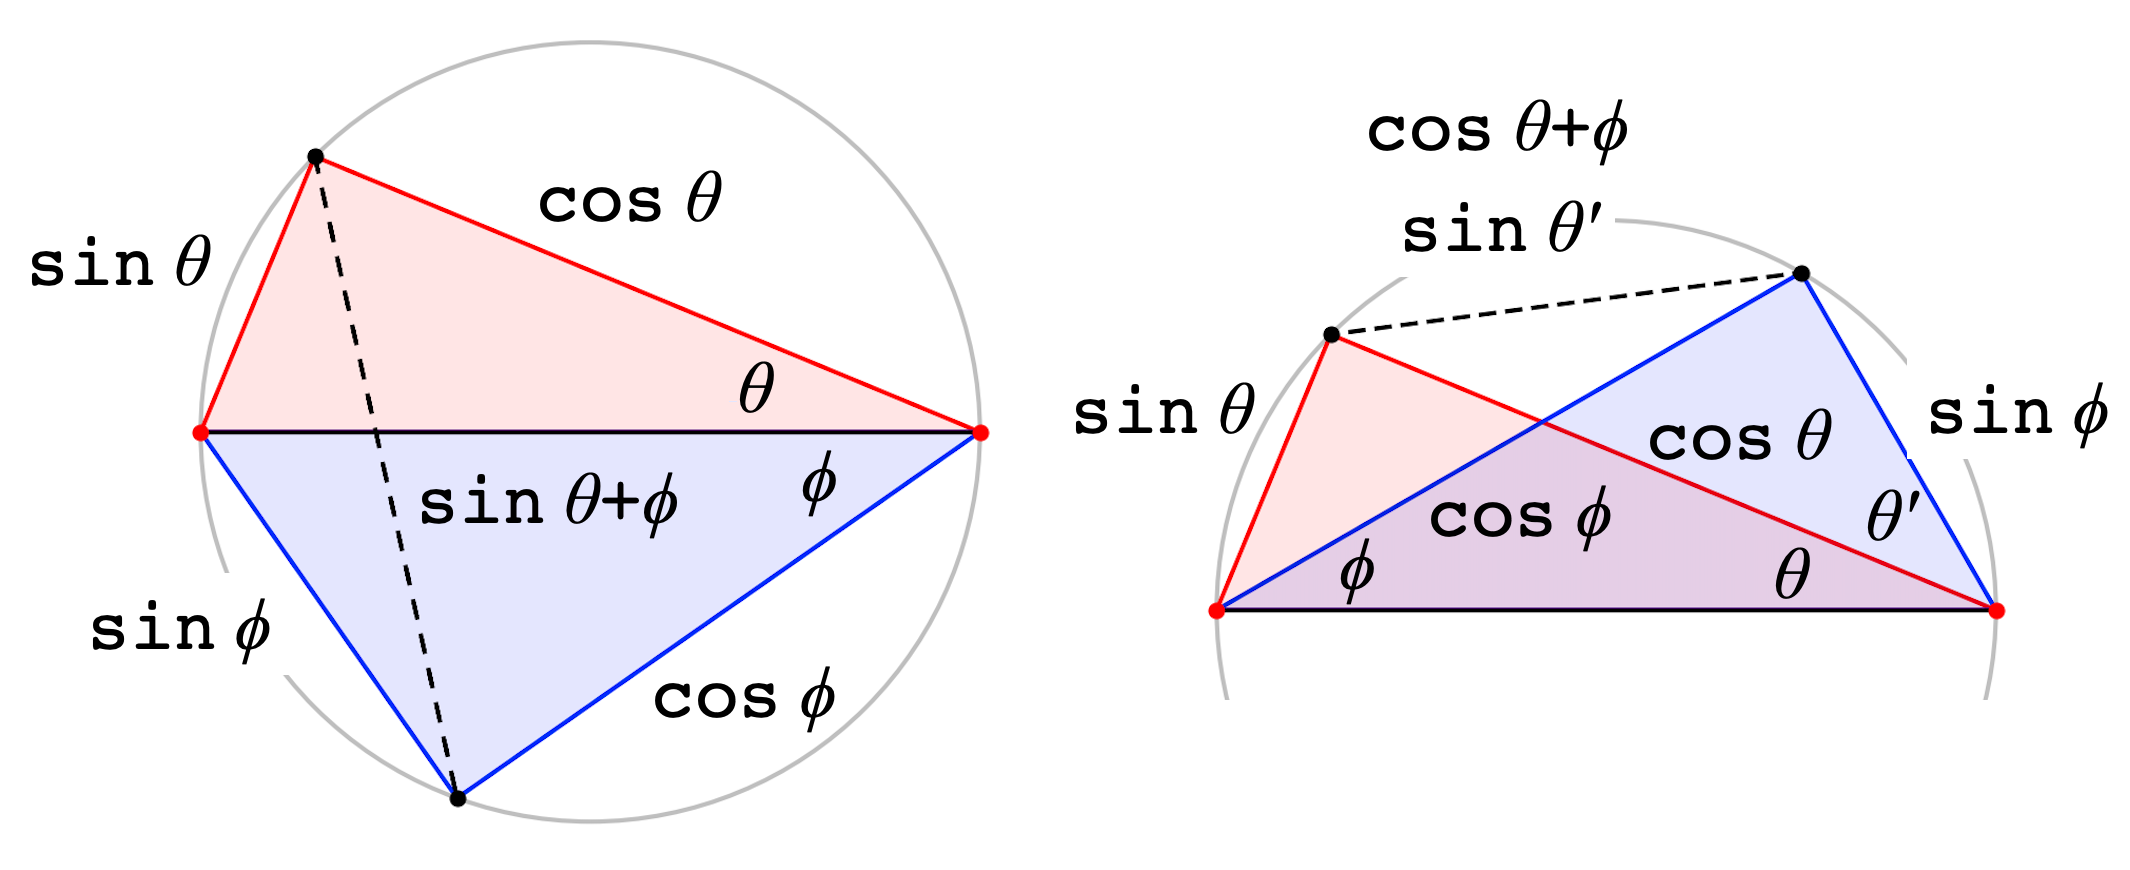
\includegraphics [scale=0.35] {sum_of_angles.png} \end{center}

Scale the circles to have unit diameter.  Then the dotted line on the left is equal to $\sin \theta + \phi$.

Ptolemy's theorem easily gives the result.
\[ \sin \theta + \phi = \sin \theta \cos \phi + \sin \phi \cos \theta \]

Similarly on the right, we have that the dotted line is $\sin \theta'$.  But $\theta'$ is complementary to $\theta + \phi$, so this is equivalent to $\cos \theta + \phi$.

\[ \sin \theta \sin \phi + \cos \theta + \phi = \cos \theta \cos \phi \]
Again , the result follows easily after rearranging.

We have assumed that the diagonal is equal to the sine of the subtended angle.  We also leave this proof as an exercise.


\end{document}